\documentclass{beamer}
\usetheme{Warsaw}
\usepackage{english}
\usepackage[utf8]{inputenc}
\usepackage[style=verbose,maxnames=99,backend=bibtex]{biblatex}
\addbibresource{bibliografia.bib}
\renewcommand{\footnotesize}{\tiny}

\title{Molding the flow of light with subwavelength elements}
\subtitle{Summary of PhD studies}
\author{Marcin Stolarek}
\institute{Information Optics Division, Faculty of Physics}
%\institute{Zakład Optyki Informacyjnej, Wydział Fizyki UW}
\date{\today}


\begin{document}
\renewcommand*{\bibfont}{\tiny}

\frame{\titlepage}

\frame{\tableofcontents}

%\section{Wielowarstwy metaliczno-dielektryczne}
\section{Metal-dielectric multilayers}
%\subsection{Pryzmat do obrazowania podfalowego}
\begin{frame}
	\begin{columns}
		\begin{column}{0.5\textwidth}
			\begin{figure}
				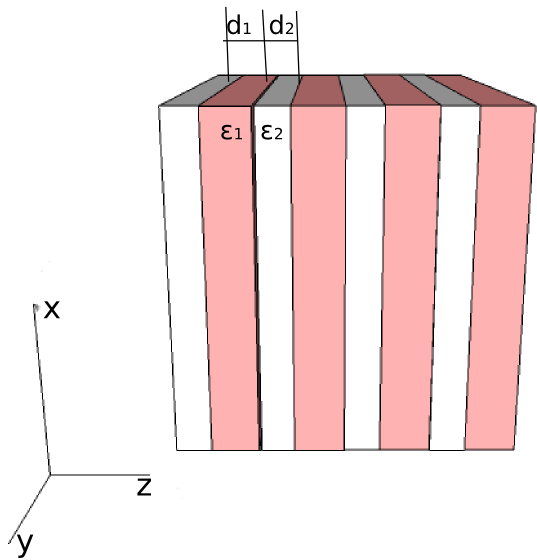
\includegraphics[width=\textwidth]{../images/multilayer/multilayer-3d.png}\\
		 	%{\tiny Do projekotwania własności wielowarstwy wykorzystywaliśmy model efektywny, do badania własności symulacje metodami macierzowymi i~FDTD.}
			
			\end{figure}
		 	{\tiny Initial design of metamaterial is based on effective medium theory and is further refined with numerical simulations ( TMM/SMM, FDTD).}
		\end{column}
		 \begin{column}{0.5\textwidth}
			\[ \varepsilon= \left[ \begin{array}{ccc}
							\varepsilon_{\parallel} & 0 & 0 \\
							0 & \varepsilon_{\parallel} & 0 \\
							0 & 0 &  \varepsilon_{\perp} \end{array} \right]
			\] 		

			\[ \mu= \left[ \begin{array}{ccc}
							\mu_{\parallel} & 0 & 0 \\
							0 & \mu_{\parallel} & 0 \\
							0 & 0 &  \mu_{\perp} \end{array} \right]
			\] 		

			$\varepsilon_{\parallel}=f\cdot{\varepsilon_1}+{1-f}\cdot \varepsilon_2$\\
			$\varepsilon_{\perp}=\left(f\cdot{\varepsilon_1^{-1}}+(1-f)\cdot \varepsilon_2^{-1}\right)^{-1}$\\
			$\mu_{\parallel}=f\cdot{\mu_1}+{1-f}\cdot \mu_2$\\
			$\mu_{\perp}=\left(f\cdot{\mu_1^{-1}}+(1-f)\cdot \mu_2^{-1}\right)^{-1}$
		\end{column}
	\end{columns}
	{\tiny {\tiny  \cite{PhysRevLett.85.3966}}}
\end{frame}

\begin{frame}
	\begin{columns}
		\begin{column}{0.5\textwidth}
			\begin{figure}
				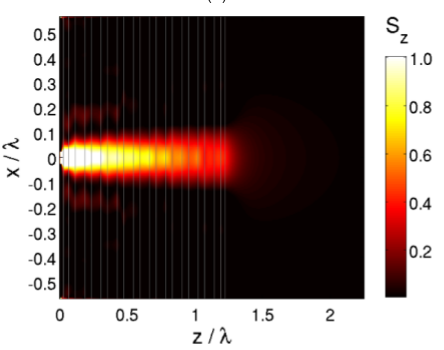
\includegraphics[width=\textwidth]{../images/multilayer/nondiffAMR.png}
		 	%{\tiny Do projekotwania własności wielowarstwy wykorzystywaliśmy model efektywny, do badania własności symulacje metodami macierzowymi i~FDTD.}
			\end{figure}
		 	{\tiny Initial design of metamaterial is based on effective medium theory and is further refined with numerical simulations ( TMM/SMM, FDTD). }
		\end{column}
		 \begin{column}{0.5\textwidth}
			\begin{itemize}
				\item for instance $\varepsilon_{\parallel}=0$, $\varepsilon_{\perp}= \infty$ 
				\item with real metamaterials we can achieve point spread function with FWHM of ~10nm
				\item two modes of operation: canalization and resonant tunneling
				\item transmission enhancement with coupling/decoupling layers, impledance matching, up to ~70\%
			\end{itemize}
					
			
		\end{column}
	\end{columns}
\end{frame}




\begin{frame}
	\begin{columns}
		\begin{column}{0.5\textwidth}
			\begin{figure}
			Fourier Optics provides us nice framework to deal with linear shift-invariant (LSI) systems. 
			\\	
			We can describe such a system with point spread function (PSF) and it's Fourier transform modulation transfer function (MTF). 
			\\
			\end{figure}
		\end{column}
		\begin{column}{0.5\textwidth}
			%{\tiny Analiza własności wielowarstwy na podstawie wyników symulacji SMM i~TMM prowadzona w~języku optyki Fourierowskiej.}
			\begin{figure}
				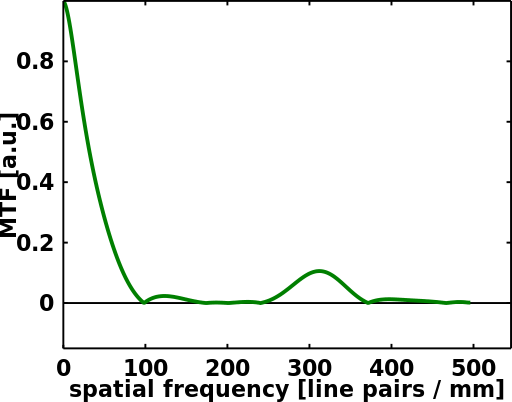
\includegraphics[width=0.5\textwidth]{images/MTF-example.png}
				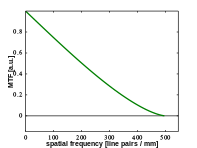
\includegraphics[width=0.6\textwidth]{images/MTF-perfect.png}
			\end{figure}
			\begin{figure}
				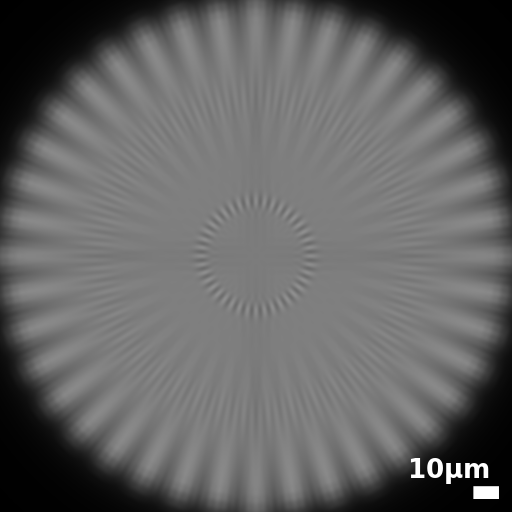
\includegraphics[width=0.5\textwidth]{images/Spoke.png}
				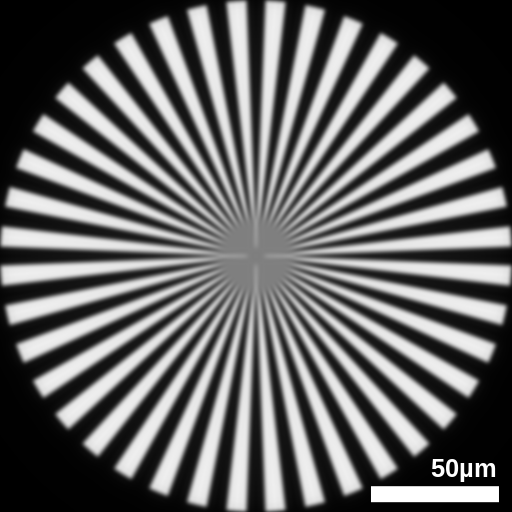
\includegraphics[width=0.5\textwidth]{images/Spoke-perfect.png}
			\end{figure}
		\end{column}
	\end{columns}
\end{frame}


\subsection{Superresolving prism}
\begin{frame}
	\begin{columns}
		\begin{column}{0.5\textwidth}
		%	Wykorzystanie pryzmatu miało umożliwić operację rzutowania również dla wiązek o~rozmiarach podfalowych.
			The aim - to couple near-field subwavelength sized field distribution and far-field images (applications in microscopy, lithography, etc)
			\begin{figure}
				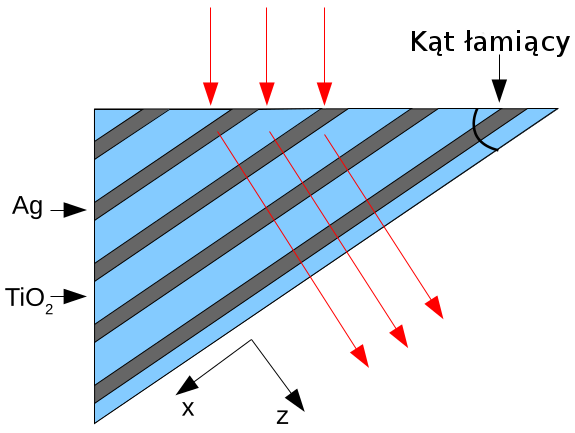
\includegraphics[width=\textwidth]{../images/multilayer/prism.png}
			\end{figure}
		\end{column}
		\begin{column}{0.5\textwidth}
		%	Wysoki współczynnik transmisji może być osiągnięty przez dopasowanie impedancyjne współczynników efektywnych do powietrza, w~przypadku rezonansowego tunelowania wysoka transmisja moze byc uzyskana przez odpowiednie dobranie grubosci calej struktury do dlugosci fali.
		High transmision coefficent can be achieved with impedance matching with surrounding media or using the resonant tunneling.

			{\tiny \cite{scalora-transparentmetal}}
		\end{column}
	\end{columns}
		
\end{frame}

\begin{frame}[t]
	\begin{columns}
		\begin{column}{0.5\textwidth}
			\begin{figure}
				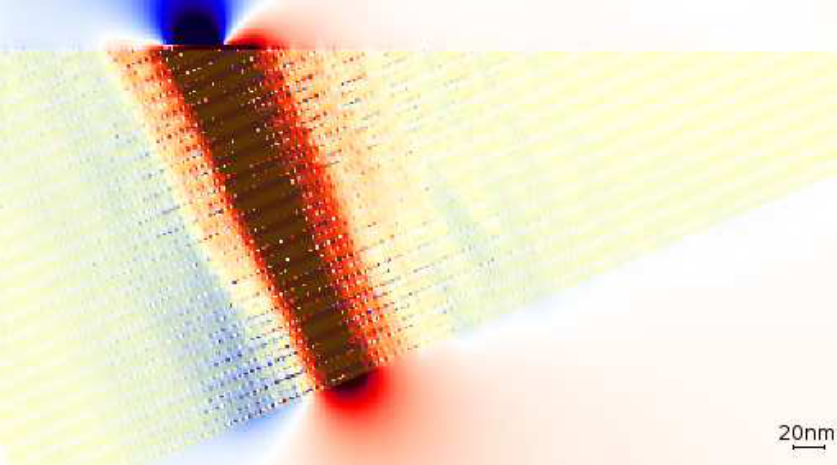
\includegraphics[width=\textwidth]{../images/multilayer/prism04.png} \\
				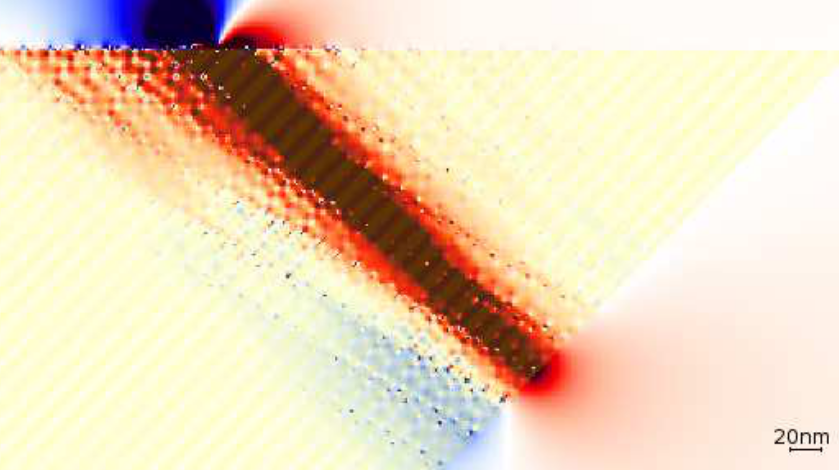
\includegraphics[width=\textwidth]{../images/multilayer/prism08.png} \\
			\end{figure}
		\end{column}
		\begin{column}{0.5\textwidth}
				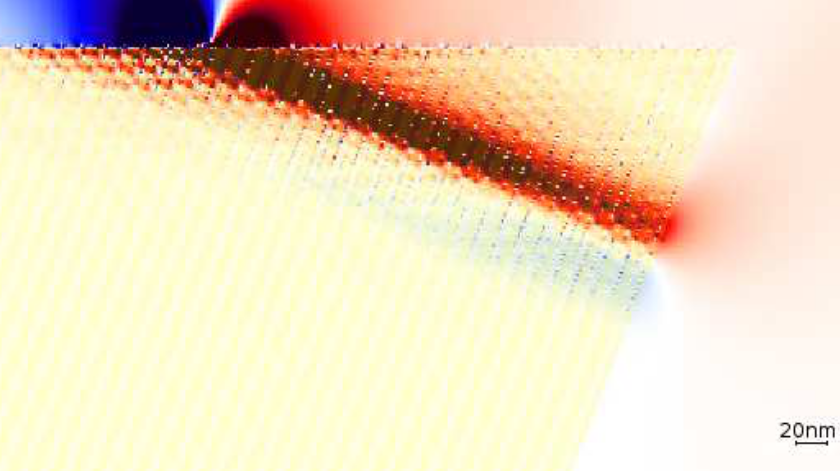
\includegraphics[width=\textwidth]{../images/multilayer/prism12.png}\\
			%	Wydajność i~FWHM wiązki wychodzącej zależą nie tylko od kąta łamiącego pryzmatu, ale i~od przesunięcia wiązki wchodzącej, wskazując na brak możliwości stosowania modelu ośrodka efektywnego we wszystkich tego typu układach.
				Transmision efficiency and FWHM of the outgoing beam depends not only on the appex angle, but also on shift of illuminating beam. (Not an LSI system)
	
		\end{column}
	\end{columns}
	{\tiny \cite{prism2010}}
		
\end{frame}

%\subsection{Projektownie układów przez ray tracing}
\subsection{Pseudo ray-tracing design}

\begin{frame}
Subwawelength beam concentrator based on metal-dielectric multilayers
	\begin{columns}
		\begin{column}{0.5\textwidth}
			\begin{figure}
				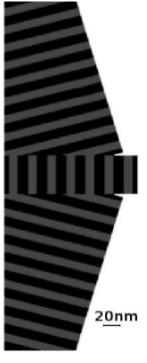
\includegraphics[angle=90,width=\textwidth]{../images/multilayer/konc_eps_mgr.png}\\
				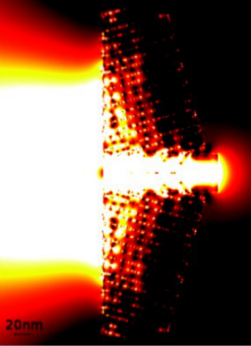
\includegraphics[angle=90,width=\textwidth]{../images/multilayer/konc_ene_mgr.png}
			\end{figure}
		\end{column}
		\begin{column}{0.5\textwidth}
			\begin{itemize}
			%	\item Inżynierski model projektowania.
				\item Simple model based on EMT and ray-tracing (good for engineeing)
			%	\item Ograniczony silną dyfrakcją poza strukturą.
				\item Limited by strong diffraction outside the structure
		%		\item Ścisłe modelowanie niezbędne.
				\item Rigorous modeling is needed to explain the appearance of resonanses, reflections and losses
			\end{itemize}
		
		\end{column}
	\end{columns}
		
\end{frame}

\begin{frame}
	\begin{columns}
		\begin{column}{0.5\textwidth}
			\begin{figure}
				Cylindrical concentrator
				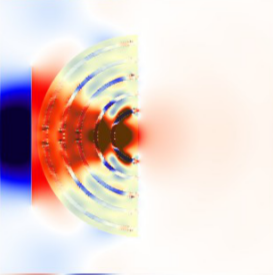
\includegraphics[width=\textwidth]{../images/multilayer/konc_polk_poynt.png}\\
			\end{figure}
		\end{column}
		\begin{column}{0.5\textwidth}
				Simillar concentrator based on core-shell's
				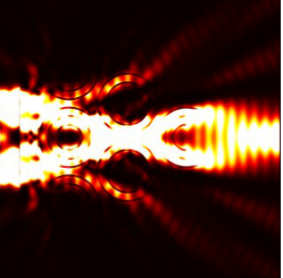
\includegraphics[width=\textwidth]{../images/multilayer/konc_coreshell_energy.png}\\
		\end{column}
	\end{columns}
		
\end{frame}

%\subsection{Wpływ gładkości warstw}
\subsection{The effect of surface roughness}
\begin{frame}
	\begin{columns}
		\begin{column}{0.5\textwidth}
			\begin{figure}
				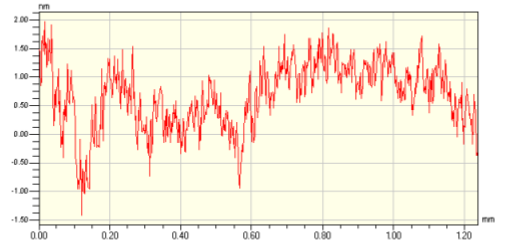
\includegraphics[width=\textwidth]{../images/multilayer/plp-afm-chropo-1d.png}\\
				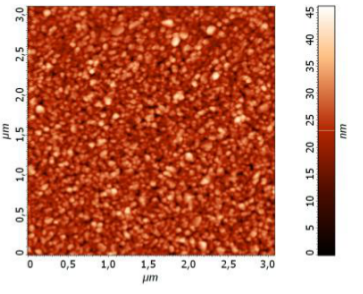
\includegraphics[width=\textwidth]{../images/multilayer/plp-afm-chropo.png}\\
			\end{figure}
		\end{column}
		\begin{column}{0.5\textwidth}
	%		Dla prowadzenia symulacji niezbędne było oddanie struktury wyspowej chropowatości powierzchni. \\ 
	%		Powierzchnie chropowate generowane były na podstawie danych z~AFM, z~zachowaniem widmowej gestosci mocy szumu.\\
		%	The crucial part of simulations was generation of similar roughness. \\
			\begin{itemize}
				\item Statistical model of surface roughness based on AFM measurements\\
				\item Rigorous FDTD simulations of rough surfaces \\
			\end{itemize}
			
		\end{column}
	\end{columns}
	{\tiny \cite{Stolarek_2013}}
		
\end{frame}

\begin{frame}
	\begin{columns}
		\begin{column}{0.5\textwidth}
			%	W symulacjach struktury w~pelni gladkiej widoczna byla stojaca fala powierzchniowa na granicy metal-dielektryk, która zanika przy wprowadzeniu nawet minimalnej chropowatości -poprawa współczynnika transmisji.\\
				The surface mode is no longer excited in the presence of surface roughness.\\
			%	Chropowatość może poprawiać PSF.\\
				Additionally roughness can improve the PSF.

		\end{column}
		\begin{column}{0.5\textwidth}
			\begin{figure}
				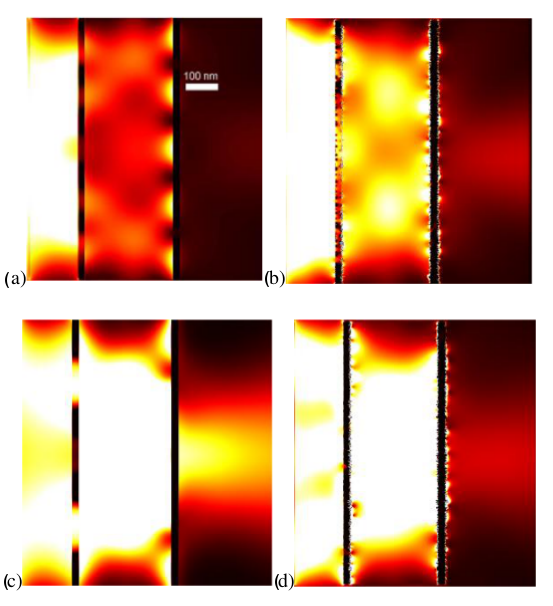
\includegraphics[width=\textwidth]{../images/multilayer/plp-chropo.png}\\
				\caption{ a,b - 430nm , c,d -490 nm}
			\end{figure}
		\end{column}
	\end{columns}
		
\end{frame}





\begin{frame}[t]
	\begin{columns}
		\begin{column}{0.5\textwidth}
			\begin{figure}
				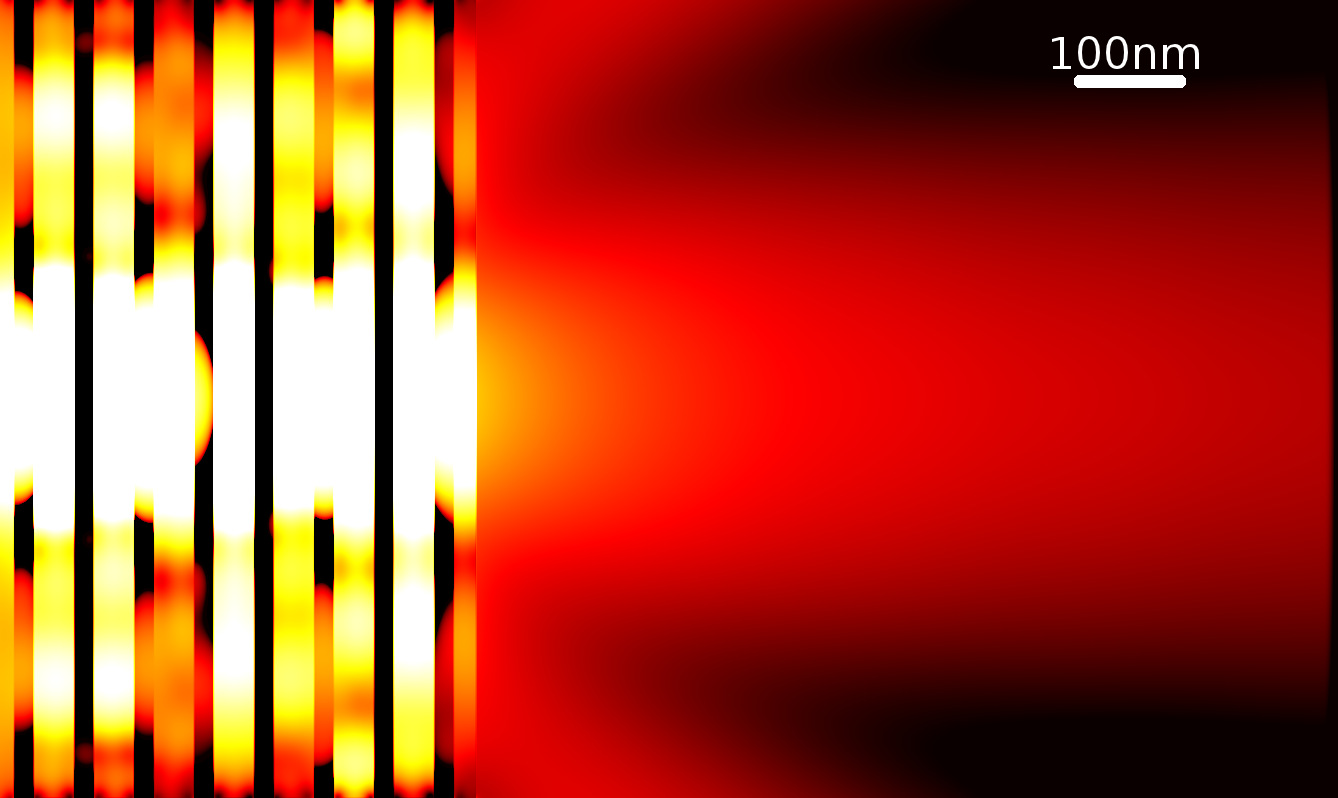
\includegraphics[width=\textwidth]{../images/multilayer/oer-rms0.png}\\
				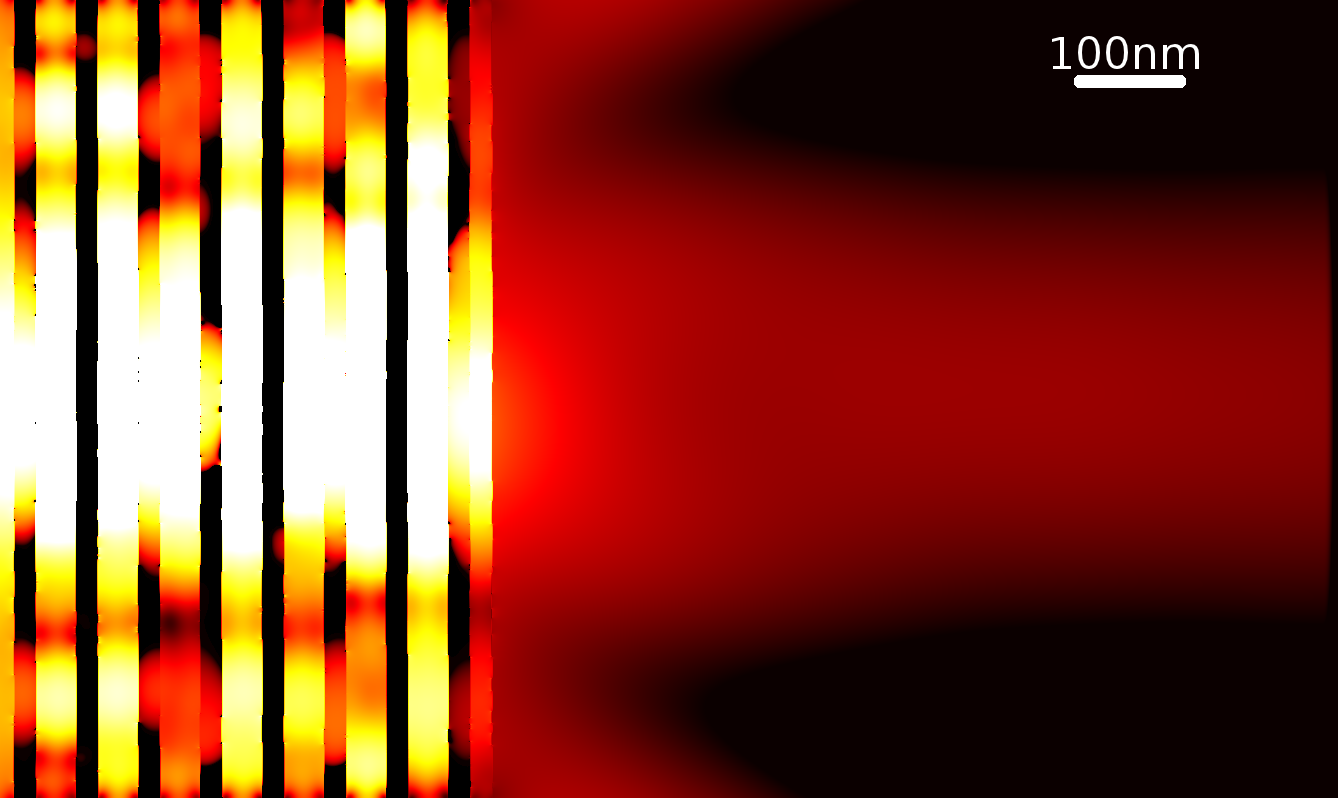
\includegraphics[width=\textwidth]{../images/multilayer/oer-rms01.png}\\
			\end{figure}
		\end{column}
		\begin{column}{0.5\textwidth}
				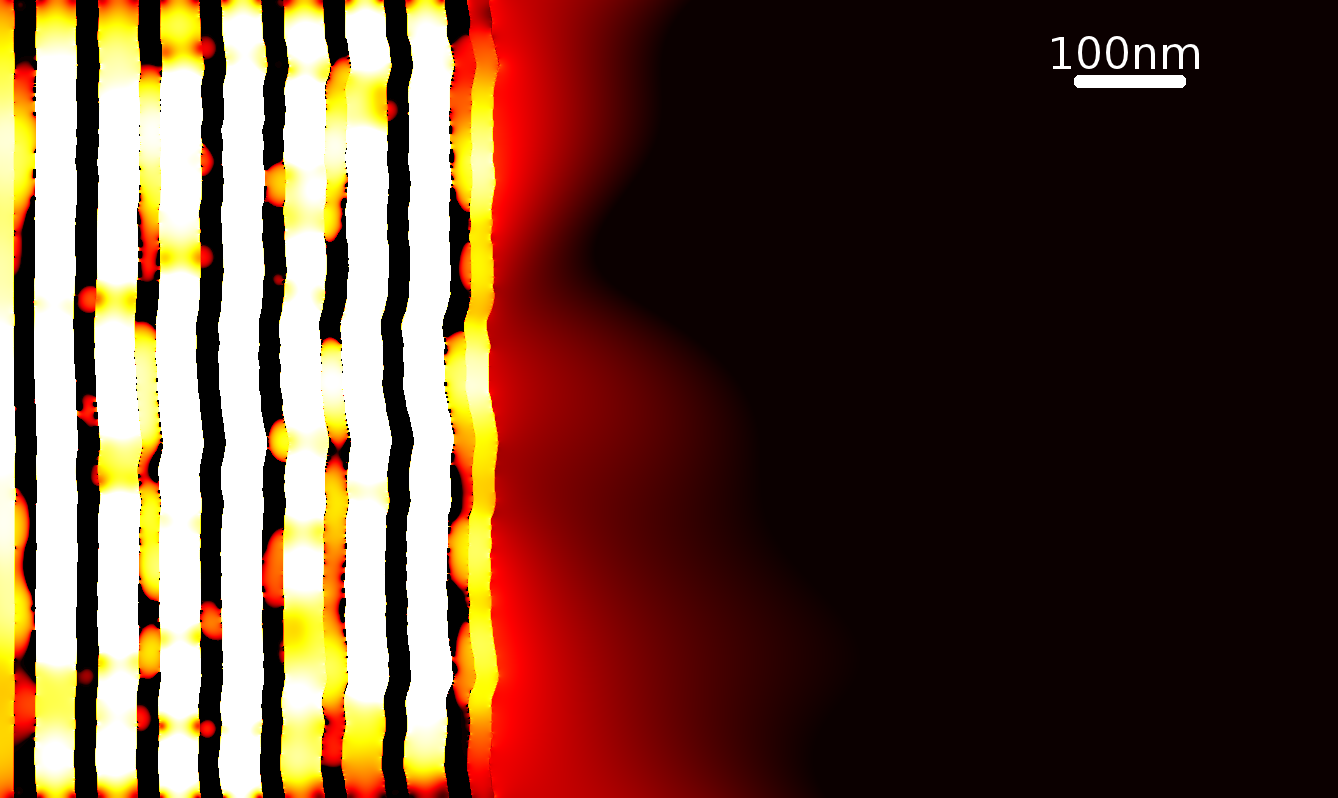
\includegraphics[width=\textwidth]{../images/multilayer/oer-rms05.png}\\
			%	Generalnie: nawet chropowatości na poziomie RMS ~ 1nm mogą znacząco zmniejszyć współczynnik transmisji przez wielowarstwę. \\
				Surface roughness of $RMS=1$~nm can significantly decrease transmission through mulitlayer structure. Especially when the number of layers is large.
			
		%		 Szczególnie w~przypadku dużej liczby warstw.
		\end{column}
	
	\end{columns}

	{\tiny \cite{pastuszczak2013engineering}}
		
\end{frame}



%\section{Siatki metalowe do kształtowania fali w~THz}
\section{Subwavelength metallic gratings for THz radiation}
%\subsection{Antena dla detektora THz}
\subsection{Antenna for THz detection}
\begin{frame}
	\begin{columns}
		\begin{column}{0.5\textwidth}
			{\tiny Theoretical maximum of transmission:}\\
			\centerline{$\frac{\lambda}{n_{eff}}=2\frac{h}{m}$}
			\begin{figure}
				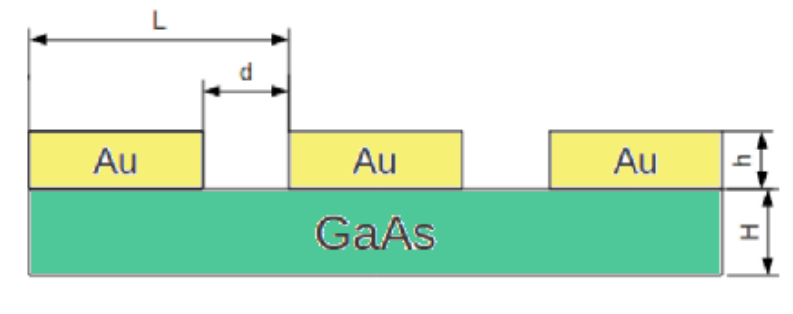
\includegraphics[width=.9\textwidth]{../images/antenaThz/schemat.png}\\
				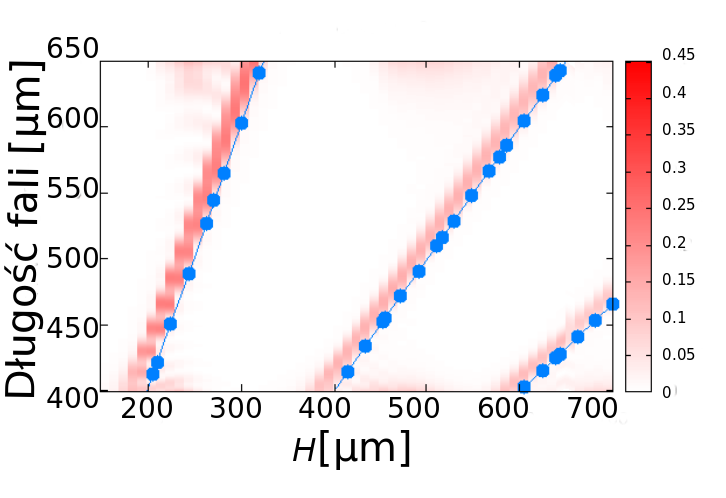
\includegraphics[width=.9\textwidth]{../images/antenaThz/rezonant_trans_f001.png}\\
			\end{figure}
		
		\end{column}
		\begin{column}{0.5\textwidth}
			\begin{figure}
				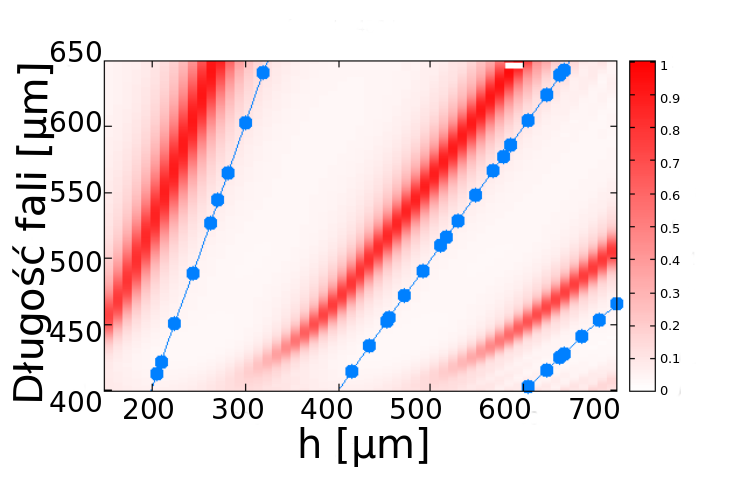
\includegraphics[width=.9\textwidth]{../images/antenaThz/rezonant_trans_f01.png}\\
				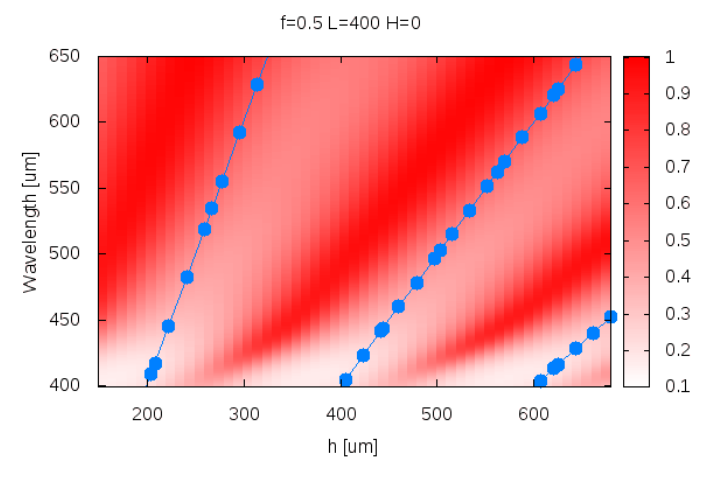
\includegraphics[width=.9\textwidth]{../images/antenaThz/rezonant_trans_f05.png}\\
			\end{figure}
		\end{column}
	\end{columns}
	{\tiny \cite{martin2001theory}	}
	
\end{frame}


\begin{frame}
	\begin{columns}
		\begin{column}{0.5\textwidth}
			\begin{figure}
				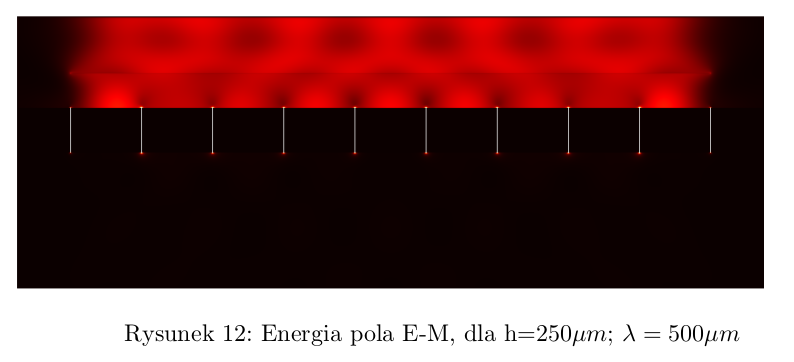
\includegraphics[width=\textwidth]{../images/antenaThz/con_src_l500.png}\\
				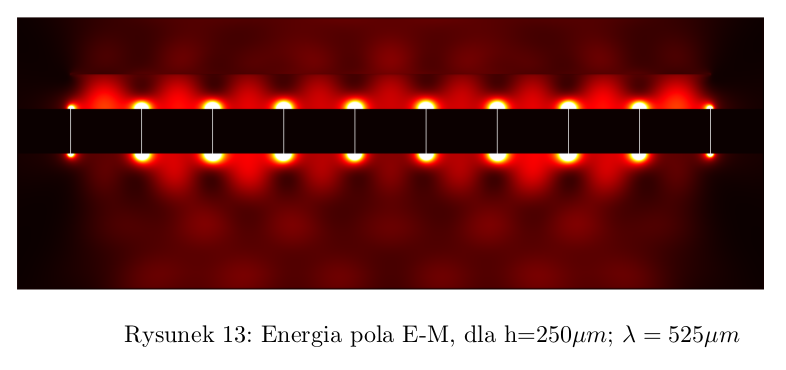
\includegraphics[width=\textwidth]{../images/antenaThz/con_src_l525.png}\\
				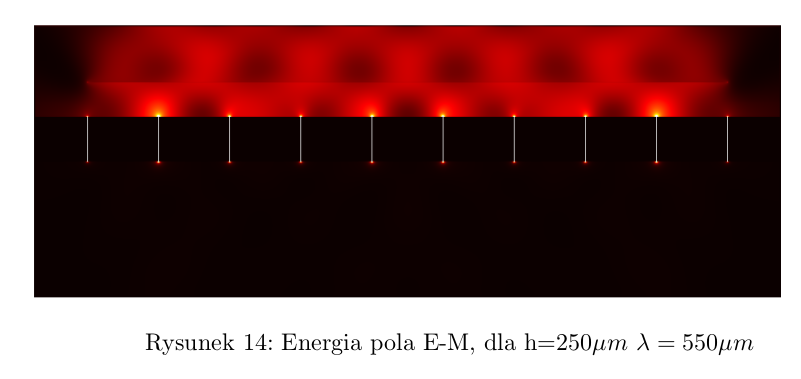
\includegraphics[width=\textwidth]{../images/antenaThz/con_src_l550.png}\\
			\end{figure}
		\end{column}
		\begin{column}{0.5\textwidth}
				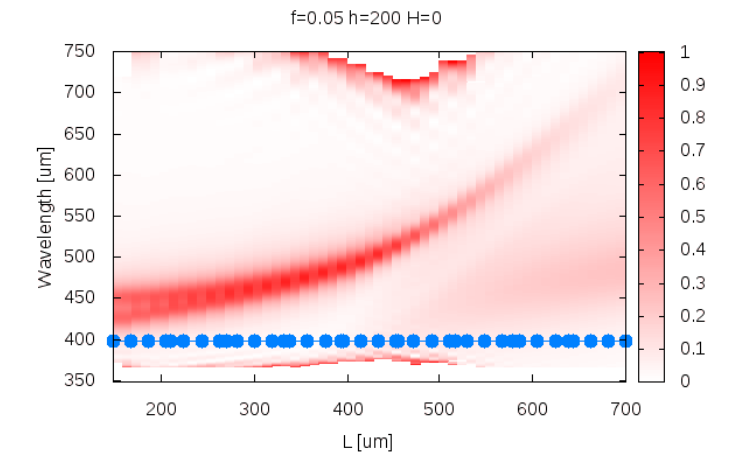
\includegraphics[width=\textwidth]{../images/antenaThz/rez_trans_L.png}\\
		%	Symulacje prowadzone byly z~roznymi modelami materialowymi, zostalo potwierdzone, że w~prowadzonych pracach metale mogą być przybliżane za pomocą PEC.
		\begin{itemize}
			\item Material properties for THz and visible light are different
			\item Frequency selective transmission due to mode coupling in a thick metallic grating
		\end{itemize}	
		\end{column}
	\end{columns}
		
\end{frame}




\begin{frame}
	\begin{columns}

		\begin{column}{0.5\textwidth}
			\begin{figure}
				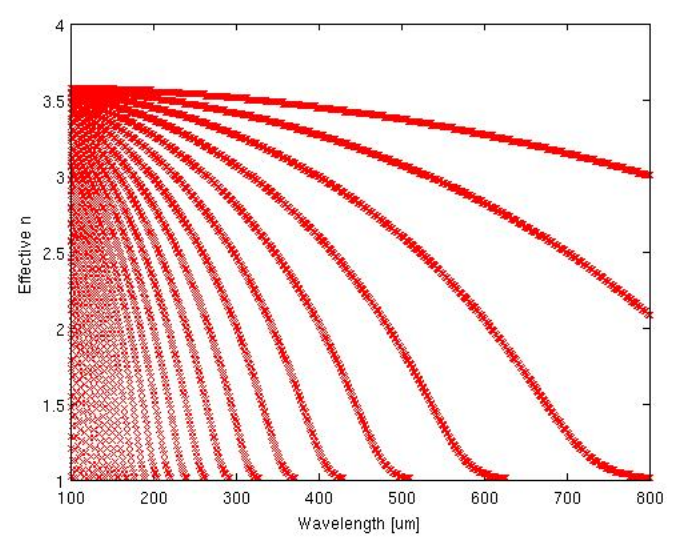
\includegraphics[width=\textwidth]{../images/antenaThz/gaas_mod_structure.png}\\
			\end{figure}
		\end{column}
		\begin{column}{0.5\textwidth}
	%		Ze względu na brak możliwości wykonania grubych siatek na podkładach GaAs zawierających detektory THz, zdecydowaliśmy się na wzbudzenie modu falowodowego w~podkładzie. Symulacje pozytywnie zweryfikowały możliwości tak zaprojektowanej anteny.
			Excitation of guided modes in GaAs with thin metallic grating
			{\tiny \cite{Stolarek2011}}
		\end{column}
	\end{columns}
	\begin{figure}
		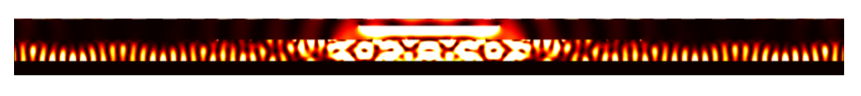
\includegraphics[width=\textwidth]{../images/antenaThz/final_stru.png}\\
	\end{figure}
	{\tiny \cite{Szczytko2012271}}
\end{frame}



%\subsection{Podwójne metalowe siatki dyfrakcyjne}
\subsection{Double metallic gratings}
\begin{frame}
Asymmetric transmission doesn't mean the device is an optical isolator.
	\begin{columns}
	\begin{column}{.5\textwidth}
		\begin{figure}
			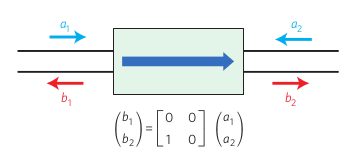
\includegraphics[width=\textwidth]{./images/simplest_isolator.png}\\
		\end{figure}
	\end{column}
	\begin{column}{.5\textwidth}
		\begin{itemize}
			\item Every system can be described in terms of scattering matrix.
			\item Backward transmission have to be blocked for ensembles of modes.
			\item If we consider only linear, time-independent and reciprocal the scattering matrix is symmetric.
			
		\end{itemize}
	\end{column}
	\end{columns}

{\tiny \cite{4171512}}
\end{frame}
\begin{frame}
	\begin{columns}
		\begin{column}{0.5\textwidth}
			\begin{figure}
				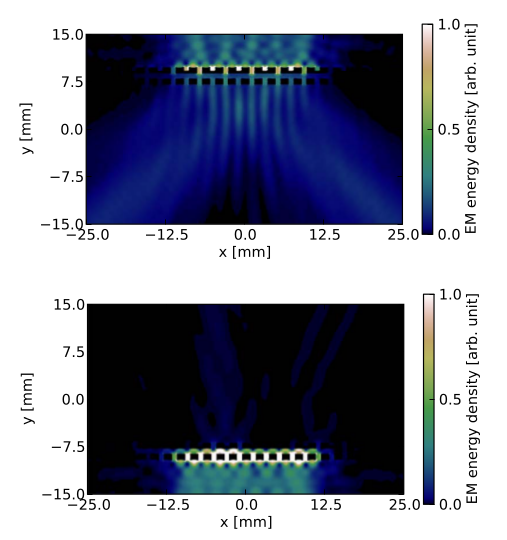
\includegraphics[width=\textwidth]{../images/dmg/letters_eneden.png}
			\end{figure}
		\end{column}
		\begin{column}{0.5\textwidth}
			$\Lambda_1 < \lambda$, $\Lambda_2 = 2 \cdot \Lambda_1 > \lambda$
			\begin{figure}
				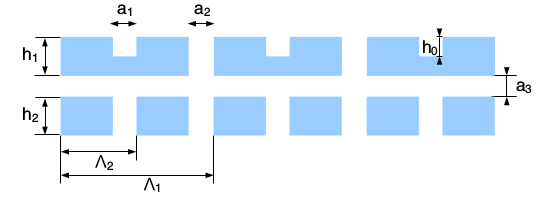
\includegraphics[width=\textwidth]{../images/dmg/letters_schemat.png}
			\end{figure}
		%	Nie jest mozliwe uzyskanie transmisji asymetrycznej przez podwójne siatki metalowe w~zerowym rzędzie ugięcia.
			The transmission assymetry is not possible in 0th diffraction order, this is reciprocal setup.
			
		\end{column}
	\end{columns}
	{\tiny \cite{Stolarek:13}}
		
\end{frame}

\begin{frame}
	\begin{columns}
		\begin{column}{0.5\textwidth}
			\begin{figure}
				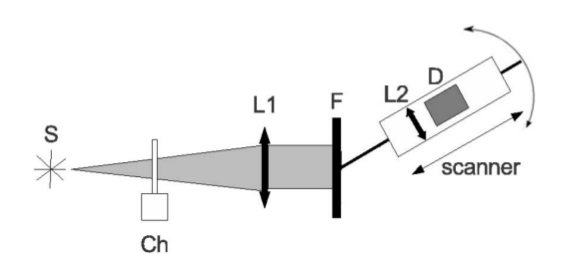
\includegraphics[width=\textwidth]{../images/dmg/letters_exp_setup.png}\\
				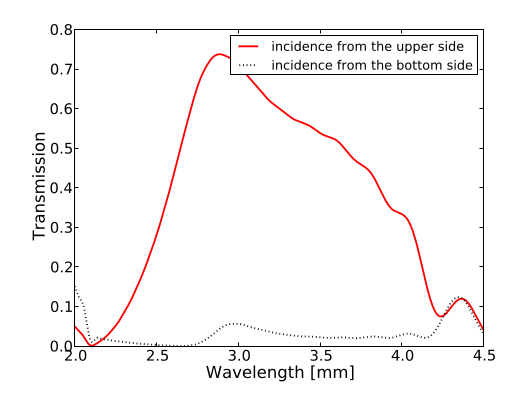
\includegraphics[width=\textwidth]{../images/dmg/letters_spect.png}\\
			\end{figure}
		\end{column}
		\begin{column}{0.5\textwidth}
				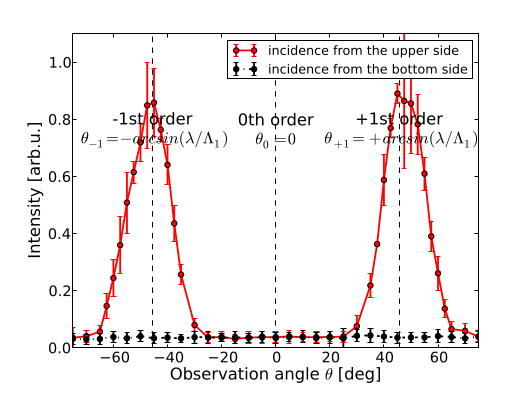
\includegraphics[width=\textwidth]{../images/dmg/letters_exp.png}\\
	%	W porównaniu do poprzednich prac na temat DMG zakres długości fali charakteryzujący się transmisją asymetryczną został znacząco powiększony.
		\begin{itemize}
			\item Optimized for a broadband operation
			\item The grating exhibits assymetric transmission in  $\pm$1st order
			\item The 0th diffraction order is blocked
		\end{itemize}
		\end{column}

	\end{columns}
		
\end{frame}

\begin{frame}
%	\frametitle{Podniesienie kontrastu}
	\frametitle{Contrast tuning}
	\begin{columns}
		\begin{column}{0.5\textwidth}
			\begin{figure}
				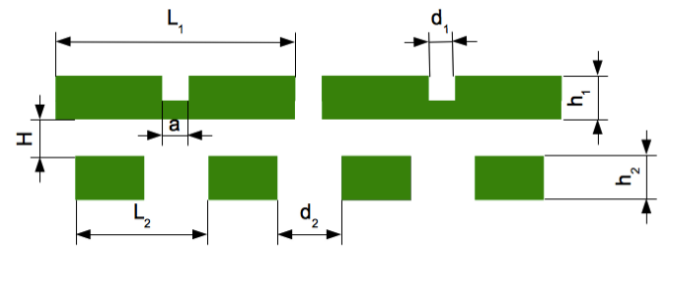
\includegraphics[width=\textwidth]{../images/dmg/kontrast_schemat.png}\\
				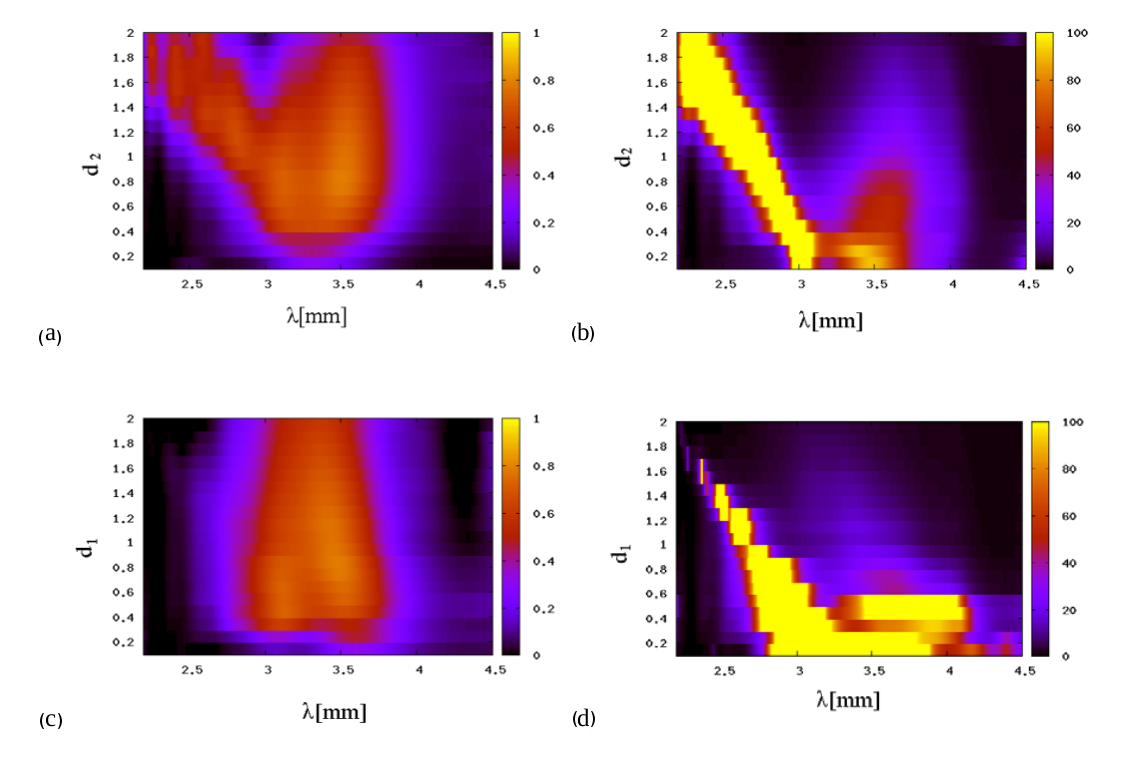
\includegraphics[width=\textwidth]{../images/dmg/kontrast_maps.png}\\
			\end{figure}
		\end{column}
		\begin{column}{0.5\textwidth}
			\begin{figure}
				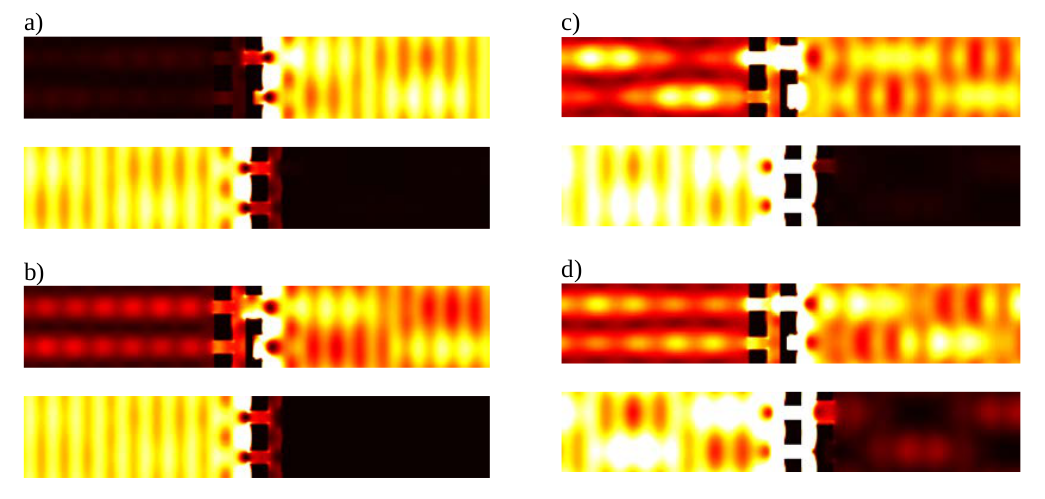
\includegraphics[width=\textwidth]{../images/dmg/kontrast_energy.png}\\
			\end{figure}
		%	Modifikacja rozmiarów otworów, oparta na zrozumieniu ich funkcji w~procesie transmisji asymetrycznej pozwoliła na osiągnięcie wyższych współczynników transmisji i~kontrastu dla propagacji w~przeciwnych kierunkach.
			The dimensions of holes and grooves is further optimized to increase the contrast between transmission in opposite directions.
			
		\end{column}
	\end{columns}
		
\end{frame}

\begin{frame}
%	\frametitle{Polaryzacja radialna}
	\frametitle{Radial polarization}
	\begin{columns}
		\begin{column}{0.5\textwidth}
			\begin{figure}
				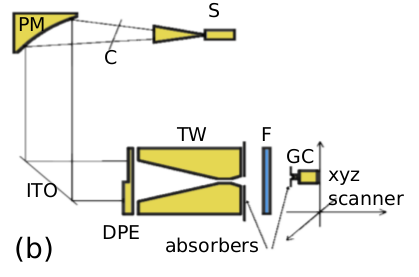
\includegraphics[width=\textwidth]{../images/dmg/express_exp_setu.png}\\
			\end{figure}
		\end{column}
		\begin{column}{0.5\textwidth}
			\begin{figure}
				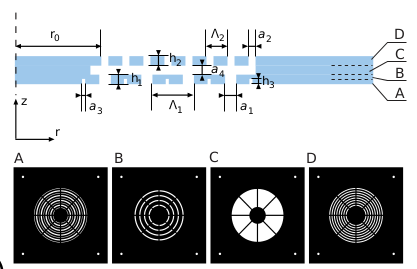
\includegraphics[width=\textwidth]{../images/dmg/express_siatki.png}\\
			\end{figure}
		\end{column}
	\end{columns}
	{\tiny \cite{Yavorskiy:14}}
		
\end{frame}

\begin{frame}
%	Struktura zaprojektowana do:
	The cylindrical double metallic grating was desinged to optimize the transmission asymmetry of a supergaussian radially polarized incident beem:
	\begin{figure}
		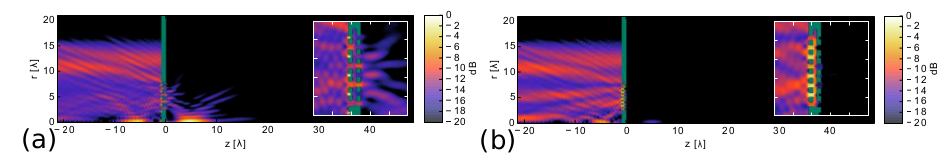
\includegraphics[width=\textwidth]{../images/dmg/express_high_contrast.png}\\
	\end{figure}
%	Eksperyment wykonany w~"przeciwnym" kierunku:
	The experimental conditions differed from the previous assumptions:
	\begin{figure}
		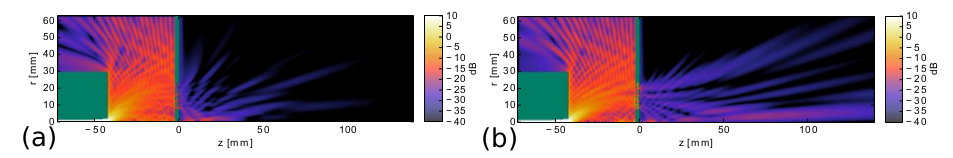
\includegraphics[width=\textwidth]{../images/dmg/express_zarmata.png}\\
	\end{figure}
		
\end{frame}

\begin{frame}
	\begin{figure}
		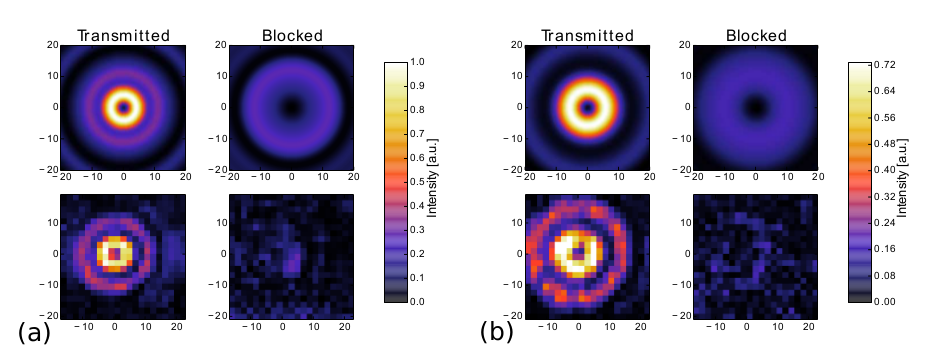
\includegraphics[width=\textwidth]{../images/dmg/express_exp.png}\\
	\end{figure}
%	Pomiary w~eksperymencie wykazuję dobrą zgodność z~modelowaniem. Oceniając wyniki eksperymentalne należy mieć na uwadze dużą wrażliwość układu na warunki zewnętrzne.
	Experimental measurements are in very good agreement with numerical modeling.
		
\end{frame}


%\section{Realizacja PML za pomocą wielowarstw}
\section{PML based on multilayers}
\begin{frame}
	\begin{figure}
				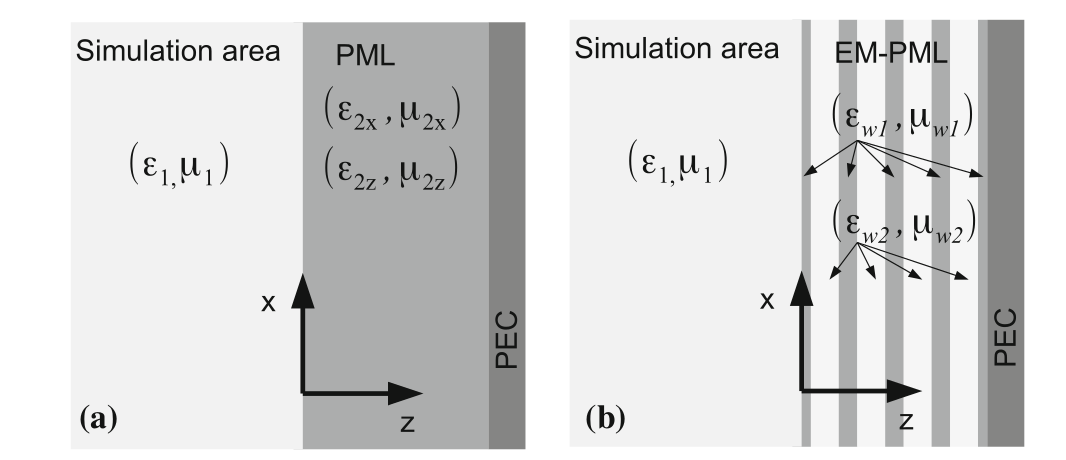
\includegraphics[width=\textwidth]{../images/pml/oqe_schemat.png}
			\end{figure}

	\begin{columns}
		\begin{column}{0.5\textwidth}

		\end{column}
		\begin{column}{0.5\textwidth}

		\end{column}
	\end{columns}
	{\tiny \cite{ania2015}	}
\end{frame}

\begin{frame}
	\begin{figure}
				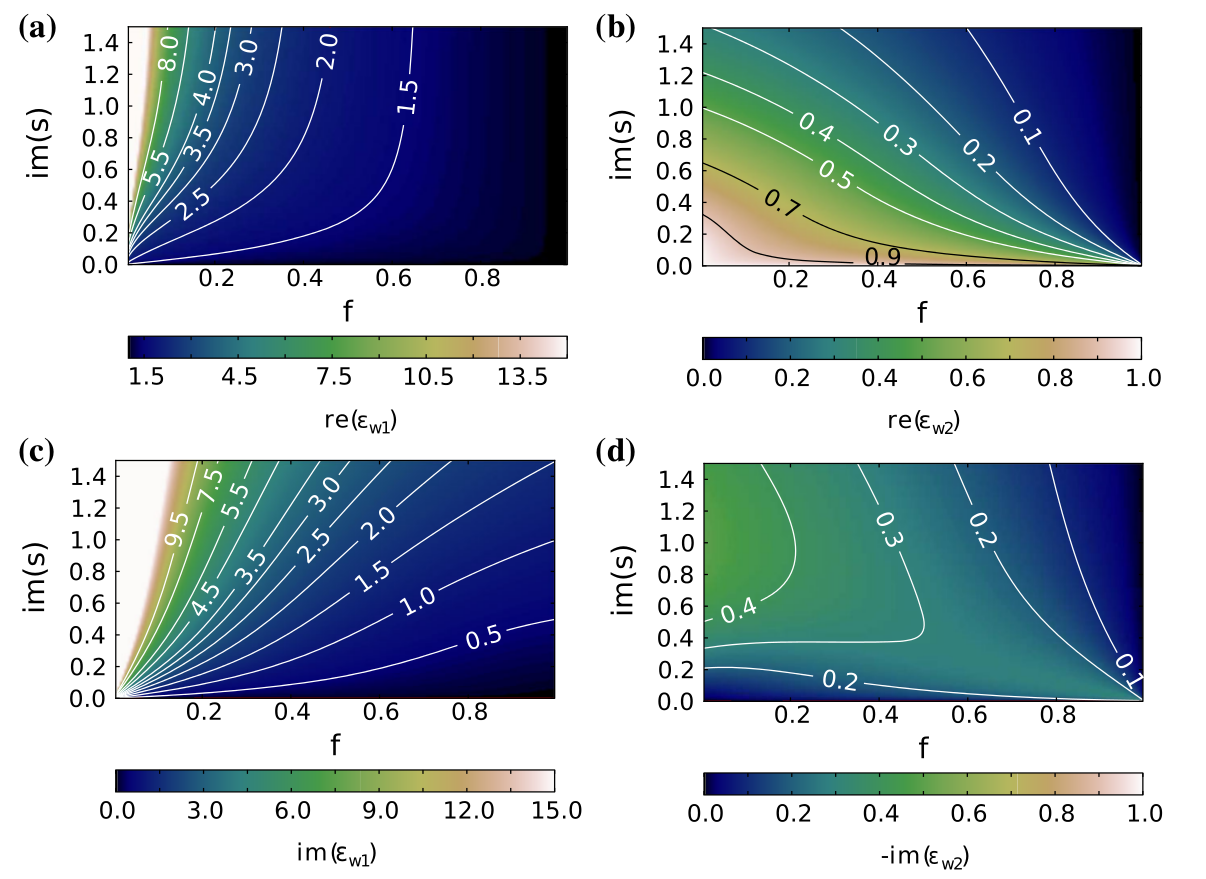
\includegraphics[width=\textwidth]{../images/pml/oqe_materials.png}
	\end{figure}
		
\end{frame}


\begin{frame} [t]
	\begin{columns}
		\begin{column}{0.5\textwidth}
			\begin{figure}
						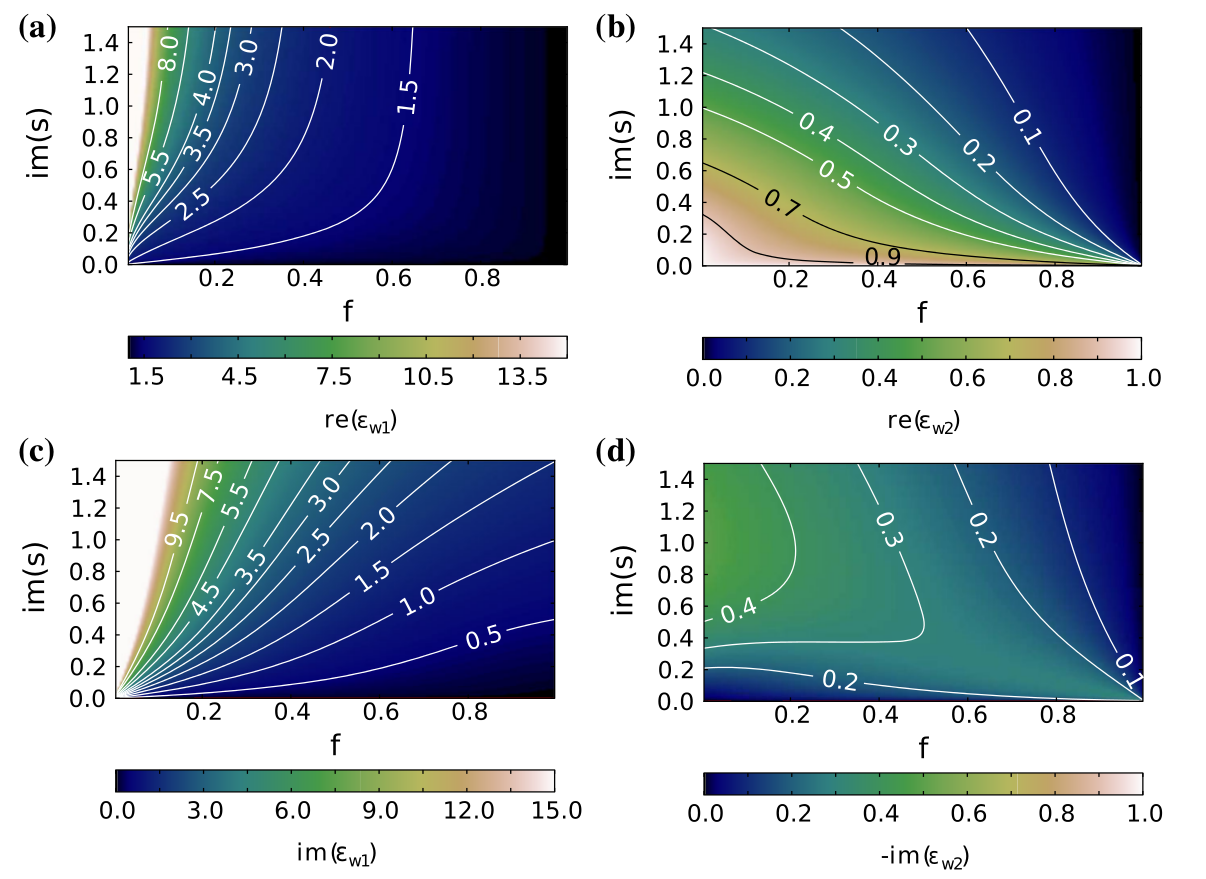
\includegraphics[width=\textwidth]{../images/pml/oqe_materials.png}
			\end{figure}
		%	Realizacja materiałw z~ $\mu \ne 1$ lub wzmocnieniem nie jest możliwa, konieczne jest przybliżenie propnowanego PML realnymi materiałami.			
			"Natural" materials with  $\mu \ne 1$ or with gain  do not exist.
		\end{column}
		\begin{column}{0.6\textwidth}
			\begin{figure}
						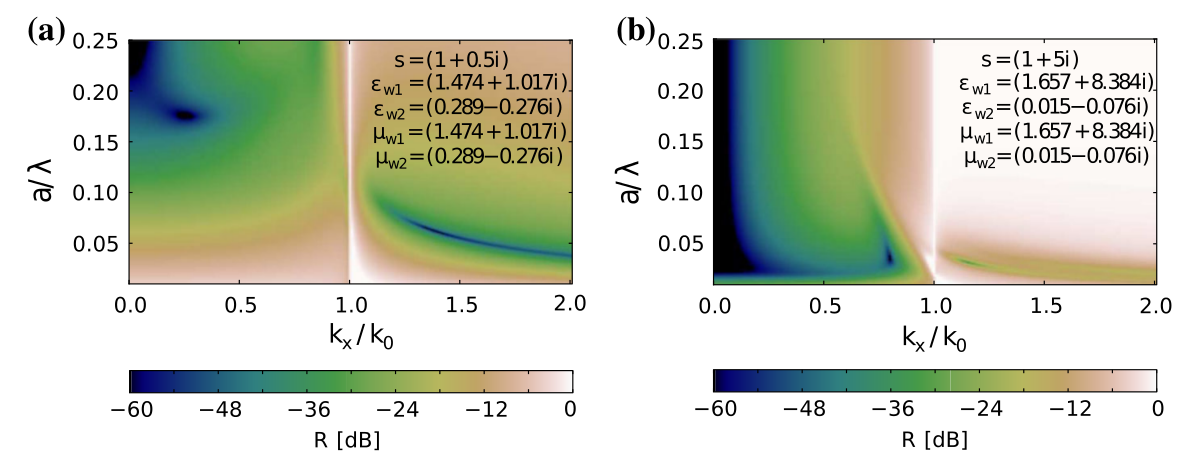
\includegraphics[width=0.9\textwidth]{../images/pml/oqe_reflection_kat.png}\\
			\end{figure}
				
%		{\tiny	Dzięki oddzielnemu rozważaniu polaryzacji możemy wykluczyć zależność od części parametrów materiałowych. Nie możemy jednak wykluczyć zespolonego charakteru $\mu$.}
		{\tiny Thaks to equation seperations for for two polarizations we can exclude the dependence from a few of material parameters, but the complex character of $\mu$ is still difficult to deal with}	

			\begin{figure}
						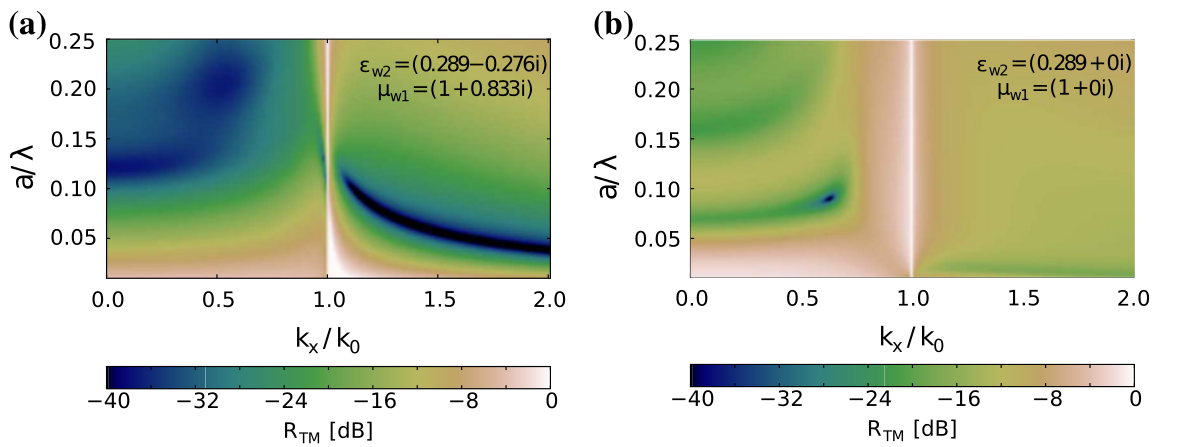
\includegraphics[width=0.9\textwidth]{../images/pml/oqe_reflection_kat_simp.png}
			\end{figure}

		\end{column}

	\end{columns}
		
\end{frame}


\begin{frame}
	\begin{columns}
			\begin{column}{0.5\textwidth}
			\begin{figure}
						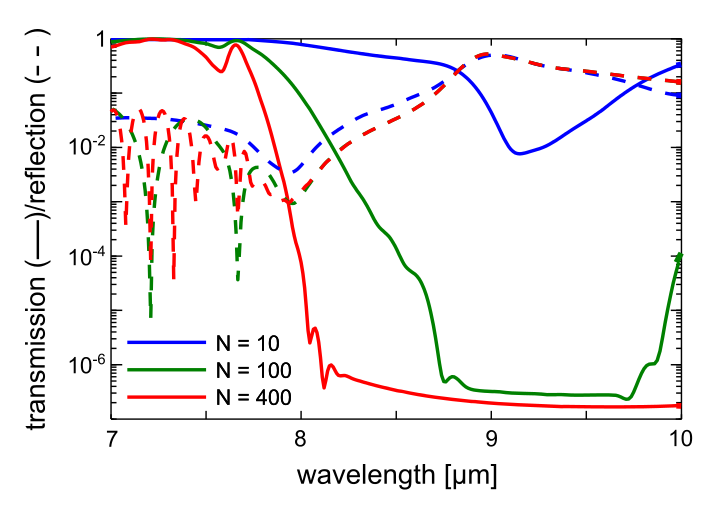
\includegraphics[width=\textwidth]{../images/pml/oqe_trans_refl.png}
			\end{figure}
		\end{column}
		\begin{column}{0.5\textwidth}
			\begin{figure}
						\includegraphics[width=1.1\textwidth]{../images/pml/oqe_coreshell.png}
			\end{figure}
		\end{column}

	\end{columns}
		
\end{frame}

\section{}

\begin{frame}
	\frametitle{Conclusions}

	\begin{itemize}
		\item Metal-dielectric multilayers with subwavelength resolutions can be used to construct different optical elements hence to the geometry modifications.
		\item It is possible to achevie asymmetric, reciprocal transmission through double mettalic grating structures in THz regime.
		\item MDMs can also be used as electromagnetic absorbers. 
	\end{itemize}

\end{frame}

%\begin{frame}
%	\frametitle{Dorobek naukowy}
%	\begin{columns}
%		\begin{column}{0.5\textwidth}
%			h-index: 3 \\
%			cited: 28 \\
%			Seamless access to the PL-Grid e-infrastructure using UNICORE middleware (7 cytowań)\\
%			Polish contribution to the worldwide LHC computing(4 cytowania)\\
%		\end{column}
%		\begin{column}{0.5\textwidth}
%			\cite{Stolarek:13}\\
%			\cite{Yavorskiy:14}\\
%			\cite{ania2015}\\
%			\cite{pastuszczak2013engineering}\\
%		\end{column}
%	\end{columns}
%		
%\end{frame}



\end{document}



%% Kawalki do przeklejania:
%% Ramka z~kolumnami i~obrazkiem:
%
